\chapter{Violación CP}\label{cap:CP_violation}
Los conceptos de paridad y violación de paridad han sido utilizados varias veces en los capítulos anteriores. Nuestro objetivo en este capítulo es proporcionar una descripción detallada de estas propiedades. Antes de comenzar con la descripción de los mesones $\PK$ neutros y la violación CP, resulta útil dar unas pinceladas sobre el concepto de paridad y qué papel jugaron los kaones en el descubrimiento de su violación en la fuerza débil. 

Cuando ciertas propiedades de una partícula no cambian al someterla a un conjunto de transformaciones, se dice que esa partícula tiene una simetría. De acuerdo con el Teorema de Noether, cada simetría se asocia a una magnitud física que se conserva, las cuales se describen mediante operadores hermíticos. Hay dos simetrías discretas importantes que conviene discutir en relación con los mesones $\PK$, ya que en la interacción fuerte y en la
electromagnética se conservan, pero pueden violarse en la interacción débil. Estas dos simetrías son la inversión espacial P y la conjugación de carga C.

En la invariancia frente a la inversión espacial o simetría P (también denominada paridad) se invierte el signo de las coordenadas espaciales de las partículas. En consecuencia, los términos pseudoescalares y los vectores polares cambian su signo (ejemplos de vectores polares son la posición $\vec{r}$ y el momento lineal $\vec{p}$), mientras que los escalares y los vectores axiales o pseudovectores lo conservan (ejemplos de vectores axiales son el momento angular orbital $\vec{l}$ o el espín $\vec{s}$). Esta simetría se describe mediante el operador paridad $\hat{P}$. La paridad intrínseca o paridad-P $\eta _{P}\left(A \right)$ se determina empíricamente y se asocia con la estructura interna de la partícula A, pudiendo ser su valores $\pm 1$. Para fermiones y bosones se tiene $\eta _{P}\left(f \right)= -\eta_{P} \left(\overline{f} \right)$ y $\eta_{P}\left(b \right)=\eta_{P}\left(\overline{b}\right)$, respectivamente \cite{notas2020}. 

De forma similar, la invariancia frente a la conjugación de carga o simetría C, transforma partículas A en antipartículas $\overline{A}$ y viceversa, de modo que cambia el signo de la carga y del resto de números cuánticos internos (número bariónico $B$, número leptónico $L$, extrañeza $S$, etc.), dejando intactos la masa, la energía, el momento y el espín.  El operador asociado es $\hat{C}$. Nuevamente, $\eta _{C}\left(A\right)= \pm 1$. En este caso, sólo las partículas neutras tienen la paridad-C  $\eta _{C}\left(A \right)$ bien definida \cite{notas2020}. 

Estas dos simetrías parecían conservarse siempre en los procesos donde intervenían interacciones fundamentales. Sin embargo, el hallazgo de los mesones $\PK$ trajo consigo las primeras evidencias de que la interacción débil podía violar las simetrías P y C.


\subsubsection{Enigma $\Ptau$-$\theta$}
Tras las primeras observaciones de los mesones $\PK$ en los años 50, existían dos procesos de decaimiento de este tipo de partículas, por entonces llamadas partículas $V$, que desconcertaban a los científicos de la época. La confusión era tal que en un principio se consideró que ambos decaimientos correspondían a partículas $V$ distintas, a las que denominaron $\Ptau$ y $\theta$, como se mencionó en el capítulo \ref{cap:strangeness}. 

Recordemos que, por una parte, en la fotografía \ref{fig:nature1}, se observaba el decaimiento $\theta^{0} \rightarrow \Ppiplus\Ppiminus$ y años más tarde también se había constatado la existencia del proceso $\theta^{+} \rightarrow \Ppiplus\Pgpz$. Por otro lado, la fotografía \ref{fig:powell} mostraba la desintegración de $\APtauon \rightarrow \Pgpp\Pgpp\Pgpm$.  El estudio de estos dos procesos concluía que las partículas $\Ptau$ y $\theta$ eran idénticas pues tenían las mismas masas, las mismas vidas medias, etc., pero dado que los decaimientos tenían distinta paridad, era \textit{imposible} que fueran las mismas partículas; no se concebía que la paridad fuera violada. Esto hecho fue conocido como el \textit{enigma $\Ptau$-$\theta$} \cite{Ferbel}. En la expresión que sigue se muestra el análisis de la paridad en ambos procesos:
\begin{equation}
\begin{gathered}
\theta^{+} \rightarrow \pi^{+}\pi^{0} \Rightarrow \eta_{P}\left(\pi^{+}\right) \eta_{P}\left(\pi^{+}\right) = 1 , \\ 
\tau^{+} \rightarrow \pi^{+}\pi^{+}\pi^{-} \Rightarrow \eta_{P}\left(\pi^{+}\right) \eta_{P}\left(\pi^{+}\right) \eta_{P}\left(\pi^{-}\right) = -1 .
\end{gathered}
\end{equation}
En 1956, Lee y Yang estudiaron a fondo estos procesos (y muchos más), concluyendo que no había ninguna evidencia para afirmar que la paridad se conservara en la interacción débil, por lo que las partículas $\tau$ y $\theta$ debían ser la misma y la violación de la paridad en esta interacción era una realidad más que plausible. 

El experimento clave que corroboró esta hipótesis, realizado por Wu y Ambler, consistió en analizar la emisión $\beta$ del $\tensor*[^{60}]{\mathrm{Co}}{}$ polarizado (por ser semejante a la del neutrón): 
\begin{equation}
\tensor*[^{60}]{\mathrm{Co}}{} \longrightarrow \tensor*[^{60}]{\mathrm{Ni}}{} + \Pem + \APnu_{e} .
\end{equation}
Utilizando un campo magnético externo, se polarizan los espines de un cristal de cobalto radioactivo previamente enfriado a $\SI{0,01}{\kelvin}$, minimizando así su despolarización por agitación térmica. Cuando el núcleo de cobalto decae, se miden las direcciones de los electrones emitidos. Wu y Ambler notaron que, preferentemente, los $\Pem$ se emitían en la dirección del campo magnético $\vec{B}$ y, por lo tanto, en la dirección del momento angular del $\tensor*[^{60}]{\mathrm{Co}}{}$. Esto es, si el campo apuntaba al norte, los $\Pem$ se emitían en esa misma dirección. Para que la paridad se conserve, si se repite el mismo experimento alineando el espín nuclear nuevamente, pero ahora en dirección sur, los $\Pem$ deberían, asimismo, salir orientados hacia el sur. No obstante, se observó que este no era el caso y los electrones seguían mostrando preferencia por emitirse en dirección norte, constatado así la violación de simetría P en la interacción débil \cite{Ferbel} \cite{Griffiths2008}. 

\begin{figure}[!ht]
\begin{subfigure}[t]{.5\textwidth}
  \centering
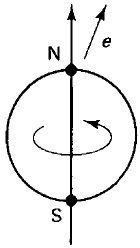
\includegraphics[width=0.4\linewidth]{{C:/Users/Carmen/Desktop/Universidad/TFG/Borradores/img/cobalto1.PNG}}
\caption{$\Pem$ emitido en la dirección del campo.}
  \label{fig:cobalto1}
\end{subfigure}%
\begin{subfigure}[t]{.5\textwidth}
  \centering
  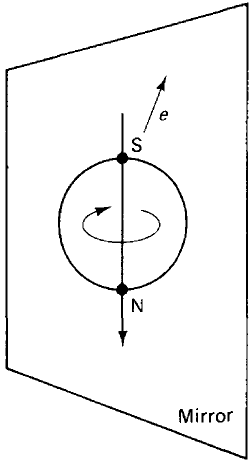
\includegraphics[width=0.45\linewidth]{{C:/Users/Carmen/Desktop/Universidad/TFG/Borradores/img/cobalto2.PNG}}
  \caption{$\Pem$ emitido dirección opuesta al campo.}
  \label{fig:cobalto2}
\end{subfigure}
\caption[Experimento de Wu y Ambler]{Evidencia de la violación P en el experimento de Wu \cite{Griffiths2008}.}
\label{fig:cobalto}
\end{figure}

Hasta mediados de los 50, los científicos consideraban que la mitad de los neutrinos tendrían helicidad positiva y la otra mitad helicidad negativa. La implicación verdaderamente importante que tuvo descubrir la violación P en la fuerza débil fue que sólo existían neutrinos con helicidad negativa y antineutrinos con helicidad positiva. 

Siguiendo la misma línea de razonamiento, si aplicásemos la conjugación de carga a un neutrino (que tiene helicidad negativa), nos daría un antineutrino. Pero como la paridad-C no cambia el espín, el $\APnu$ resultante mantendría la helicidad negativa del $\Pnu$ original. Y ya hemos confirmado mediante el experimento de Wu que esto no es posible, pues sólo existen antineutrinos con helicidad positiva. Por ende, la interacción débil también presenta violación de simetría C.

Tras descubrir que la fuerza débil no respetaba las simetrías P y C e intentando unificar las propiedades de las fuerzas fundamentales, se formuló que la combinación de ambas simetrías o simetría CP era lo que realmente debía conservarse.

No obstante, en 1964, el estudio de los decaimientos de mesones $\PKz$ evidenció la violación CP en la interacción débil. La siguiente sección presenta una descripción detallada del decaimiento de los mesones $\PKz$, la violación CP y sus implicaciones.
\vspace{5mm}

\section{Decaimiento de mesones $\PK$ neutros}
\label{sec:neutral_kaon_decay}
Volvamos a la época entre 1953 y 1955, relatada en el capítulo \ref{cap:strangeness}. El concepto de extrañeza acababa de surgir y la propuesta de Nishijima se basaba en clasificar los mesones $\PK$ en dobletes de carga, uno para las partículas $\PKp$ y $\PKz$ asignándoles un valor de extrañeza $S=1$, y otro para las correspondientes antipartículas $\PKm$ y $\PaKz$, con $S=-1$.

La teoría parecía clara pero, en el laboratorio, ¿cómo es posible distinguir $\PKz(S=1)$ de $\PaKz(S=-1)$? Esta pregunta, planteada por Fermi, obtuvo su respuesta al formularse un nuevo concepto: los \textit{estados mixtos} (o \textit{mezcla}) de las partículas.

Recordemos que los mesones $\PK$ son los mesones más ligeros que contienen el quark $\Pqs$ y se producen por interacción fuerte. Por ello, $\PKz\left(\Pqd\Paqs\right) $ y $\PaKz\left(\Pqs\Paqd\right)$ son autoestados de la interacción fuerte (autoestados de extrañeza), pero se denominan estados de sabor. Sin embargo, ya vimos que los mesones $\PK$ únicamente decaen mediante interacción débil. Esta última interacción es la que permite mezclar los kaones neutros, tal y como se muestra en la figura \ref{fig:kaonmix}. Para entender esta nueva hipótesis sobre ``mezcla de partículas'', utilizamos el mismo ejemplo que expone Pais en su libro \cite{Pais}:

Si al decaimiento $\PKz \rightarrow \Pgpp + \Pgpm$, con amplitud A, le aplicamos una conjugación de carga C, el decaimiento resultante es $\PaKz \rightarrow \Pgpp + \Pgpm$, también de amplitud A. Se observa que el estado final es el mismo para ambos procesos, pero el inicial no, al tener diferente extrañeza. Esto es debido a que la extrañeza no tiene por qué conservarse en la fuerza débil. Entonces, se tiene que $\PKz$ y $\PaKz$ se mezclan como $\PKz \leftrightarrows \Pgpp + \Pgpm \leftrightarrows \PaKz$.

\begin{figure}[!ht]
	\centering
	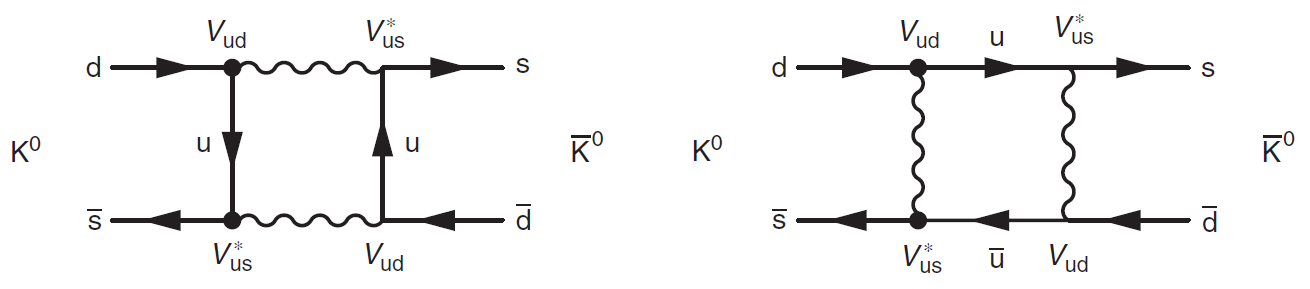
\includegraphics[width=0.85\textwidth]{C:/Users/Carmen/Desktop/Universidad/TFG/Borradores/img/mixing.png}
	\caption[Diagrama de Feynmann de la mezcla de mesones $\PK$ neutros]
	{Diagrama de Feynman de la mezcla de mesones $\PK$ neutros \cite{Thomson}.}
	\label{fig:kaonmix}
\end{figure}

Según explica Thomson en su libro \cite{Thomson}: ``Los estados físicos en mecánica cuántica son autoestados del hamiltoniano de una partícula libre. Hasta el momento, sólo se han usado estados estacionarios independientes para describir cada partícula. Sin embargo, debido a la mezcla entre $\PKz \leftrightarrow \PaKz$, según se propague $\PKz$, puede transformarse en $\PaKz$, y viceversa. Por esta razón, el sistema $\PKz \leftrightarrow \PaKz$ debe considerase como un todo.'' Los estados físicos del mesón $\PK$ neutro son los estados estacionarios del hamiltoniano combinado del sistema $\PKz \leftrightarrow \PaKz$. Luego, los kaones neutros se propagan como combinaciones lineales de los estados de sabor $\PKz$ y $\PaKz$, del tipo $|K\rangle=\alpha|\PKz\rangle+\beta|\PaKz\rangle$. Esta combinaciones conforman los estados físicos que se propagan, conocidos como kaón de vida corta $\PKzS$ (``\textit{short-lived}'' o ``\textit{$\PK$-shor}t'') y kaón de vida larga $\PKzL$ (``\textit{long-lived}'' o ``\textit{$\PK$-long}''). Por lo tanto, los mesones $\PK$ neutros se propagan como las partículas físicas $\PKzS$ y $\PKzL$, las cuales tienen modos de decaimiento y vidas medias diferenciados. Experimentalmente, $\tau\left(\PKzL\right) \approx 570 \tau\left(\PKzS\right)$ \cite{Zyla}:
\begin{align}
\tau\left(\PKzS\right) &= \SI{8,954(4)e-11}{\second}, & \tau\left(\PKzL\right) &= \SI{5,116(21)e-8}{\second}.
\end{align}

Además, estudios empíricos posteriores indicaron que la masa de $\PKzL$ es ligeramente mayor que la de $\PKzS$ (ver eq. \ref{eq:massdiff}). Esta diferencia es ínfima en comparación con las masas de $\PKzS$ y $\PKzL$ (o $\PKz$ y $\PaKz$) que son del orden de $\SI{500}{\MeV}.$
Al tener masas bien definidas, $\PKzS$ y $\PKzL$ también se designan como autoestados de masa \cite{Thomson}.
\begin{equation}
\Delta m= m\left(\PKzL\right)-m\left(\PKzS\right)=\SI{3,5e-12}{\MeV}.\label{eq:massdiff}
\end{equation}

Si la interacción débil fuera invariante frente a la simetría CP, los estados físicos $\PKzS$ y $\PKzL$ serían equivalentes a los autoestados CP del mesón $\PK$ neutro. Cabe destacar que esta fue la suposición inicial, pues todo este desarrollo fue concebido varios años antes al descubrimiento de la violación P y C en la interacción débil. De este modo, haciendo uso de los operadores $\hat{P}$, $\hat{C}$ y $\hat{C}\hat{P}$, se tiene:
\begin{align}
\hat{P}|\PKz\rangle &= -|\PKz\rangle & \hat{P}|\PaKz\rangle &= -|\PaKz\rangle\\
\hat{C}|\PKz\left(\Pqd\Paqs\right)\rangle &= e^{i\zeta}|\PaKz\left(\Pqs\Paqd\right)\rangle & \hat{C}|\PaKz\left(\Pqs\Paqd\right)\rangle &= e^{i\zeta}|\PKz\left(\Pqd\Paqs\right)\rangle ,
\end{align}
donde $\zeta$ es un factor de fase no observable. Por convenio, se toma $\zeta=\pi$ \cite{Thomson}, por lo que:
\begin{align}
\hat{C}|\PKz\left(\Pqd\Paqs\right)\rangle &=|\PaKz\left(\Pqs\Paqd\right)\rangle & \hat{C}|\PaKz\left(\Pqs\Paqd\right)\rangle &= |\PKz\left(\Pqd\Paqs\right)\rangle\\
\hat{C}\hat{P}|\PKz\rangle &= +|\PaKz\rangle & \hat{C}\hat{P}|\PaKz\rangle &= +|\PKz\rangle .
\end{align}

Por consiguiente, se definen las siguientes combinaciones como autoestados de CP:
\begin{align}
|\PK_{1}\rangle &= \dfrac{|\PKz\rangle + |\PaKz\rangle}{\sqrt{2}}, & |\PK_{2}\rangle &= \dfrac{|\PKz\rangle - |\PaKz\rangle}{\sqrt{2}}.\label{eq:k1k2def}
\end{align}

Esto implicaba que, \textit{considerando} que la paridad conjunta CP se conserve en la interacción débil, $\PK_{1} \equiv \PKzS$ sólo puede decaer en estados pares, es decir, con CP=+1, mientras que $\PK_{2} \equiv \PKzL$ sólo decae a estados impares con CP=-1. Así, $\PK_{1}$ puede decaer a $\Pgpp \Pgpm$ (con amplitud $A/ \sqrt{2}$) pero $\PK_{2}$ no (amplitud nula). En consecuencia, $\PK_{1}$ y $\PK_{2}$ tienen vidas medias diferentes $\tau_{1}$ y $\tau_{2}$, respectivamente \cite{Pais} \cite{Perkins}.

Dado que, típicamente, la designación de partícula se asigna a aquellos estados físicos con una semivida definida, es más correcto expresar los estados de sabores como combinaciones lineales de los autoestados CP \cite{Pais}:
\begin{align}
|\PKz\rangle &= \dfrac{|\PK_{1}\rangle + |\PK_{2}\rangle}{\sqrt{2}}, & |\PaKz\rangle &= \dfrac{|\PK_{1}\rangle - |\PK_{2}\rangle}{\sqrt{2}}.\label{eq:k1k2defbuena}
\end{align}
No obstante, ambas combinaciones de estados (\ref{eq:k1k2def} y \ref{eq:k1k2defbuena}) pueden utilizarse dependiendo del proceso específico que estemos analizando.

Generalmente, los mesones $\PK$ neutros decaen por interacción débil en dos o en tres piones (además de en estados semi-leptónicos). Al comienzo de este capítulo, comentábamos en el enigma $\Ptau$-$\theta$ que el modo $2\Pgp$ tiene P=+1 y CP=+1 mientras que el de $3\Pgp$ tiene P=-1 y CP=-1 (ambos procesos tienen C=+1). Luego, se concluyó que $\PK_{1}$ decae siempre en $2\Pgp$ mientras $\PK_{2}$ lo hace en $3\Pgp$, suponiendo que la simetría CP fuera exacta. Ahora, dado que la desintegración en $2\Pgp$ es mucho más abundante y más rápida porque libera más energía que el modo $3\Pgp$, tiene una vida media más corta, así $\tau_{2} \gg \tau_{1}$. 

Puesto que, como se ha indicado anteriormente, la masa de $\PKzL$ es levemente mayor que $\PKzS$, $\PKzL$ es más pesado y no se mueve tan rápidamente como $\PKzS$. No obstante, la mayor estabilidad de $\PKzL$ permitía explicar que su alcance fuera mayor ($\tau\left(\PKzL\right)\equiv \tau_{2}$ mayor que $\tau\left(\PKzS\right) \equiv \tau_{1}$). De hecho, esto era lo que los científicos observaban en el laboratorio: únicamente distinguían entre un kaón de vida corta y un kaón de vida larga.

Sin embargo, al año siguiente, en 1956, se resolvió el enigma $\Ptau$-$\theta$ descubriéndose la violación de paridad P y C en la interacción débil y postulando que la simetría invariante era la CP. El escepticismo acerca de esta hipótesis estaba presente en la comunidad científica. Por ello, durante los siguientes años, se estudiaron en profundidad los distintos modos de decaimiento de los mesones $\PK$ neutros, analizando la invariancia CP.

En 1964, el grupo de Cronin y Fitch, obtuvo la primera evidencia de violación CP en la interacción débil al observar un decaimiento de $\PKzL$ en dos piones: $\PKzL \rightarrow \Pgpp\Pgpm$ \cite{Cronin}.

El experimento que descubrió la violación CP consistía en una fuente que emitía un haz de kaones neutros, el cual seguidamente era colimado y atravesaba un tubo largo. Como se ha comentado anteriormente, $\PKzL$ puede alcanzar una mayor distancia de propagación al tener una semivida mayor que $\PKzS$. Esto implica que al detector situado en el extremo final del tubo únicamente llegaba un haz de mesones $\PKzL$ puro. La gran mayoría de desintegraciones detectadas eran decaimientos en $3\pi$. Sin embargo, también midieron algunos decaimientos de $\PKzL$ en $2\pi$. Los modos $\PKzL \rightarrow 2\Pgp$ eran muchísimo menos numerosos; de un total de $\num{22700}$ decaimientos detectados, sólo $\num{45 \pm 9}$ correspondían al modo $2\Pgp$ \cite{Cronin}. Además, estos procesos se caracterizaban porque el valor de CP a ambos lados de los mismos no coincidía, ergo se violaba la simetría CP:
\begin{align}
CP\left(\PKzL\right) &=-1, & CP\left(\Pgpp\Pgpm\right) &= +1.
\end{align}

La violación CP se observa en el formalismo de los mesones $\PK$ neutros de formas distintas. La primera de ellas consiste en una \textit{violación CP indirecta}. En este caso, la violación CP se produce durante el proceso de mezcla entre $\PKz \leftrightarrow \PaKz$. Nótese que la ecuación (\ref{eq:kLkSmix}) indica que los estados $\PKzS$ y $\PKzL$ no son autoestados puros de CP\protect\footnotemark , sino que se redefinen como una combinación de los autoestados $\PK_{1}$ y $\PK_{2}$, para incluir una pequeña parte $\epsilon$ del otro autoestado CP \cite{Thomson}:
\begin{align}
|\PKzS\rangle &= \dfrac{1}{\sqrt{1+\left| \epsilon\right| ^{2}}}\left( \left| \PK_{1}\rangle +\epsilon \right| \PK_{2}\rangle \right), &
|\PKzL\rangle &= \dfrac{1}{\sqrt{1+\left| \epsilon\right| ^{2}}}\left( \left| \PK_{2}\rangle +\epsilon \right| \PK_{1}\rangle \right),\label{eq:kLkSmix}
\end{align}
donde $\epsilon$ es un parámetro (número complejo) que mide la desviación de la invariancia CP en la mezcla y cuyo valor se determina empíricamente: $\num{2.228(11)e-3}$ \cite{Zyla}.

\footnotetext{Recordemos que antes de descubrir la violación CP, se pensaba que los autoestados de masa $\PKzS$ y $\PKzL$ eran equivalentes a los autoestados CP $\PK_{1}$ y $\PK_{2}$, respectivamente.}

La otra posibilidad es que la violación CP se produzca durante el decaimiento (\textit{violación CP directa}). En este caso sí se mantiene la correspondencia entre los autoestados CP y los autoestados de masa $\PKzS \equiv \PK_{1}$ y $\PKzL \equiv \PK_{2}$. La intensidad de la violación en la desintegración se parametriza mediante $\epsilon '$, siendo $\epsilon '=\Gamma\left(\PK_{2}\rightarrow \Pgp\Pgp \right) / \Gamma\left(\PK_{2}\rightarrow \Pgp\Pgp\Pgp \right)$. 

Experimentalmente, se ha demostrado que la violación directa de CP contribuye en menor medida que la indirecta \cite{Thomson}:
\begin{equation}
\Re\left(\dfrac{\epsilon '}{\epsilon}\right)=\num{1.66(23)e-3}.
\end{equation}

Aparte de en los kaones neutros, la violación CP no se volvió a observar en otras partículas hasta el descubrimiento de los mesones $\PB$ y $\PD$. Su efecto es tan pequeño que aún no se ha encontrado una manera ``natural'' de incluirlo en el formalismo débil, pero hay varias teorías. En el Modelo Estándar, una de ellas se basa en definir la fase $\delta$ de la matriz CKM como compleja para incluir los efectos producidos por la violación CP. Pese a ello, aún no hay una forma unívoca de determinar este factor ni el resto de elementos de la matriz CKM \cite{Griffiths2008}.

Los decaimientos más comunes de $\PKzS$ y $\PKzL$ se muestran en las siguientes tablas:

\begin{table}[!htb]
\begin{minipage}{.5\linewidth}
    \centering
\begin{tabular}{ c c } 
\toprule
\makecell{Mesón $\PKzS$}  &  $BR$ \\
\midrule   
$\Pgpp\Pgpm$ & $69.2\%$ \\
$\Pgpz\Pgpz$ & $30.7\%$ \\
$\Pgpz\Pgpz\Pgpz$ & $<\num{2.6e-8}$ \\
$\Pgpp\Pgpm\Pgpz$ & $\num{3.5e-7}$ \\ \hdashline
$\Pgppm\Pemp\Pnue$ & $\num{7.04e-4}$ \\
$\Pgppm\Pmump\Pnum$ & $\num{4.69e-4}$ \\
\bottomrule
\end{tabular}
\caption[Modos de decaimiento de $\PKzS$]{Modos y $BR$ de $\PKzS$ \cite{Thomson}\cite{Zyla}.}
\label{tab:KpzS_decay}
\end{minipage}\hfill
\begin{minipage}{.5\linewidth}
    \centering
\begin{tabular}{ c c } 
    \toprule
    \makecell{Mesón $\PKzL$}  &  $BR$ \\    
    \midrule
$\Pgpp\Pgpm$ & $0.20\%$ \\
$\Pgpz\Pgpz$ & $0.09\%$ \\
$\Pgpz\Pgpz\Pgpz$ & $19.5\%$ \\
$\Pgpp\Pgpm\Pgpz$ & $12.5\%$ \\ \hdashline
$\Pgppm\Pemp\Pnue$ & $40.55\%$ \\
$\Pgppm\Pmump\Pnum$ & $27.04\%$ \\
    \bottomrule
\end{tabular}
\caption[Modos de decaimiento de $\PKzL$]{Modos y $BR$ de $\PKzL$ \cite{Thomson}\cite{Zyla}.}
\label{tab:KpzL_decay}
\end{minipage}
\end{table}

Otro gran ejemplo donde se aprecia la violación CP es en los decaimientos semileptónicos de $\PKzL$. En la tabla \ref{tab:KpzL_decay} se observa que alrededor de un $33\%$ de los mesones $\PKzL$ decaen en tres piones pero otro $40\%$ lo hacen, o bien en $\Pgpm\Pep\Pnue$ o en $\Pgpp\Pem\APnue$. Nótese que si al primer proceso se le aplica una operación CP se obtiene el segundo. Si la simetría CP fuera invariante, ambos modos semileptónicos serían equiprobables. Sin embargo, los datos experimentales parecen indicar que $\PKzL$ muestra una leve preferencia por decaer en el $\Pep$ sobre el $\Pem$, permitiendo discernir entre materia y antimateria claramente. Este hecho sugiere que la violación CP puede ser responsable de que predomine la materia sobre la antimateria en el universo \cite{Griffiths2008}. No obstante, la violación CP en kaones no es lo suficientemente relevante para explicar esta asímetría. Aquí entran en juego los neutrinos. 

Los estudios más recientes en Física de Partículas se centran en estudiar las oscilaciones de neutrinos u \textit{oscilaciones de sabor} (un leptón, originalmente de un determinado sabor o familia $e$, $\mu$ o $\tau$, puede cambiar a otros sabores distintos al propagarse). En este caso, se ha comprobado que el impacto de la violación CP es mayor que en los kaones neutros, principalmente, por dos motivos. El primero ya se ha comentado y se debe a que el efecto de violación CP en mesones $\PK$ es mínimo. La otra razón tiene que ver con la limitación temporal que supone el rápido decaimiento de mesones $\PK$ frente a los neutrinos, pues los neutrinos no decaen y abundan más que los kaones en el Universo. La violación CP provoca que un $\Pnum$ se transforme en un $\Pnue$ con mucha mayor frecuencia de la que un $\APnum$ lo hace en un $\APnue$, o viceversa. De hecho, por cada 90 oscilaciones $\Pnum\rightarrow\Pnue$, se producen 15 $\APnum\rightarrow\APnue$ \cite{T2K}, ilustrando claramente la asimetría materia-antimateria.

\subsection{Oscilaciones de mesones $\PK$}\label{sec:kaon_oscillations}
Se ha comprobado que los mesones $\PK$ neutros se originan como autoestados de sabor y decaen de la misma forma (modos semi-leptónicos) o como autoestados CP (modos hadrónicos), debido al efecto de mezcla, pero se propagan como autoestados de masa. Este hecho, resulta en un fenómeno que sucede independientemente de la violación CP, conocido como \textit{oscilaciones extrañas} o \textit{de sabor} (análogamente para los neutrinos) \cite{Thomson}.

Las oscilaciones de sabor se miden gracias a los modos de desintegración semileptónicos de kaones neutros, pues son una muestra directa de la composición de quarks de estos mesones \cite{Thomson}. Esto se aprecia en los diagramas de Feynman de la siguiente figura:
\begin{figure}[!ht]
	\centering
	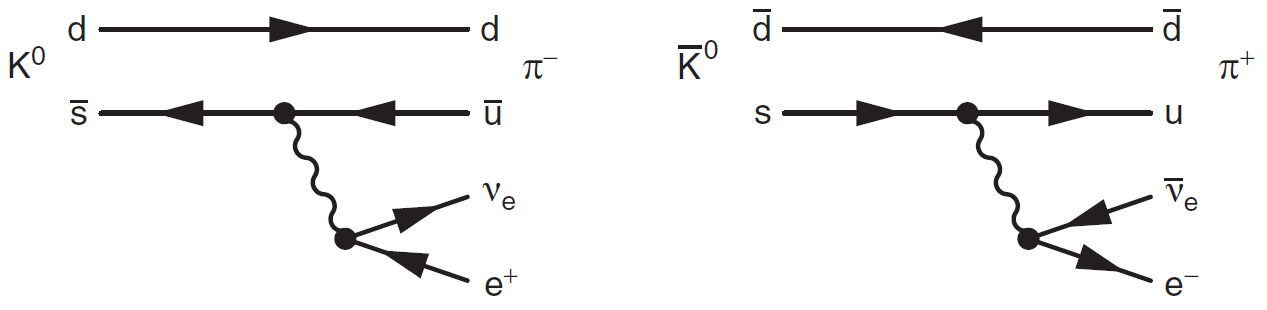
\includegraphics[width=0.65\textwidth]{C:/Users/Carmen/Desktop/Universidad/TFG/Borradores/img/osci1.PNG}
	\caption[Modos semileptónicos del electrón de mesones $\PK$ neutros]
	{Modos semileptónicos del electrón de mesones $\PK$ neutros \cite{Thomson}.}
	\label{fig:oscillation1}
\end{figure}

De acuerdo con la mecánica cuántica, la evolución temporal para $\PKzS$ y $\PKzL$ en el sistema de referencia en reposo, viene dado por:
\begin{align}
|\PKzS\left(t\right)\rangle &= |\PKzS\rangle e^{-\left(im_{S}-\Gamma_{S}/2\right)t} = \theta_{S}|\PKzS\rangle , \\
|\PKzL\left(t\right)\rangle &= |\PKzL\rangle e^{-\left(im_{L}-\Gamma_{L}/2\right)t} = \theta_{L}|\PKzL\rangle , \label{eq:evtempKSKL}
\end{align}
con $m_{S}$ y $m_{L}$ las respectivas masas de $\PKzS$ y $\PKzL$, y $\theta_{S}=e^{-\left(im_{S}-\Gamma_{S}/2\right)t}$ y $\theta_{L}=e^{-\left(im_{L}-\Gamma_{L}/2\right)t}$. Asimismo, $\tau\left(\PKzS\right) \equiv \tau_S$ y $\tau\left(\PKzL\right) \equiv \tau_L$, luego $\Gamma_{S}=1/ \tau_S$ y $\Gamma_{L}=1/\tau_L$. 

Despreciando el impacto de violación CP por ser un efecto muy pequeño ($\epsilon \approx 0$), y suponiendo un haz puro de $\PKz$, se define la evolución temporal del estado de sabor $|\PKz\rangle$ como:
\begin{equation}
|\PK\left(t\right)\rangle=\dfrac{1}{\sqrt{2}}\left(\theta_{S}|\PKzS\rangle + \theta_{L}|\PKzL\rangle \right) \approx \dfrac{1}{2}\left(\theta_{S}+\theta_{L}\right)|\PKz\rangle + \dfrac{1}{2}\left(\theta_{S}-\theta_{L}\right)|\PaKz\rangle .
\end{equation}

Como las masas $m\left(\PKzL\right) \equiv m_{L}$ y $m\left(\PKzS\right) \equiv m_{L}$ son ligeramente diferentes, las partes oscilatorias de $\theta_{L}$ y $\theta_{S}$ serán distintas también, permitiendo así que un haz puro de $\PKz$ desarrolle una componente $\PaKz$ \cite{Thomson}.

La probabilidad (o intensidad) de oscilación para cada partícula es:
\begin{align}
P\left(\PKz_{t=0} \rightarrow \PKz_{t}\right)&= |\langle\PKz|K\left(t\right)\rangle|^2 =\dfrac{1}{4}|\theta_{S}+\theta_{L}|^2 ,\label{eq:prob1osci}\\
P\left(\PKz_{t=0} \rightarrow \PaKz_{t}\right)&= |\langle\PaKz|K\left(t\right)\rangle|^2 =\dfrac{1}{4}|\theta_{S}-\theta_{L}|^2 ,\label{eq:prob2osci}
\end{align}
donde $|\theta_{S} \pm \theta_{L}|^2=|\theta_{S}|^2+|\theta_{L}|^2 \pm 2\Re\left(\theta_{S}\theta_{L}^{\ast}\right)$, siendo $|\theta_{S}|^2=e^{-\Gamma_{S} t}$ y $|\theta_{L}|^2=e^{-\Gamma_{L} t}$. 

El último término $2\Re\left(\theta_{S}\theta_{L}^{\ast}\right)$ puede reescribirse como $2\Re\left(e^{-\left(\Gamma_{S}+\Gamma_{L}\right)t/2-i\Delta mt}\right)$, y aplicando la identidad de Euler, queda: $2e^{-\left(\Gamma_{S}+\Gamma_{L}\right)t/2} \cos \left(\Delta mt\right)$, donde $\Delta m = m_{L}-m_{S}$.

Sustituyendo el resultado previo en las ecuaciones (\ref{eq:prob1osci}) y (\ref{eq:prob2osci}), se obtiene:
\begin{align}
P\left(\PKz_{t=0} \rightarrow \PKz_{t}\right) &= \dfrac{1}{4}[e^{-\Gamma_{S}t}+e^{-\Gamma_{L}t}+ 2e^{-\left(\Gamma_{S}+\Gamma_{L}\right)t/2} \cos \left(\Delta mt\right)],\label{eq:int1} \\
P\left(\PKz_{t=0} \rightarrow \PaKz_{t}\right) &= \dfrac{1}{4}[e^{-\Gamma_{S}t}+e^{-\Gamma_{L}t}-2e^{-\left(\Gamma_{S}+\Gamma_{L}\right)t/2} \cos \left(\Delta mt\right)].\label{eq:int2}
\end{align}

Estas últimas expresiones de las probabilidades de oscilación son parecidas a las de los de neutrinos. Se diferencian en que, para los mesones $\PK$ neutros, la amplitud de la oscilación disminuye a un ritmo definido por la media aritmética de $\Gamma_{S}$ y $\Gamma_{L}$.

Sabiendo que $\Delta m = \SI{3,5e-6}{\eV}$, se calcula el periodo de oscilación:
\begin{equation}
T=\dfrac{2\pi\hbar}{\Delta m} \simeq \SI{1.18e-9}{\second}.
\end{equation}

Se aprecia que $T>\tau_{S}$, por lo que, tras un sólo periodo de oscilación, $\PKzS$ y las componentes oscilatorias (\ref{eq:int1}) y (\ref{eq:int2}) habrán decaído completamente, quedando únicamente un haz puro de $\PKzL$. Por ende, la estructura oscilatoria no es muy pronunciada.  No obstante, el estudio de oscilaciones de sabor en los mesones $\PK$ neutros proporciona una herramienta muy útil para determinar $\Delta m$ \cite{Thomson}. La diferencia de masas entre $\PKzS$ y $\PKzL$ es equivalente a la rapidez con que $\PKz$ oscila a $\PaKz$ y, esto, se debe a efectos de segundo orden de la interacción débil \cite{Perkins}. La figura \ref{fig:oscillation2} muestra la evolución de la probabilidad o intensidad de cada componente $\PKzS$ y $\PKzL$ en el tiempo durante la propagación de un haz que, originalmente, sólo estaba formado por mesones $\PKz$ \cite{Thomson}. 

\begin{figure}[!ht]
	\centering
	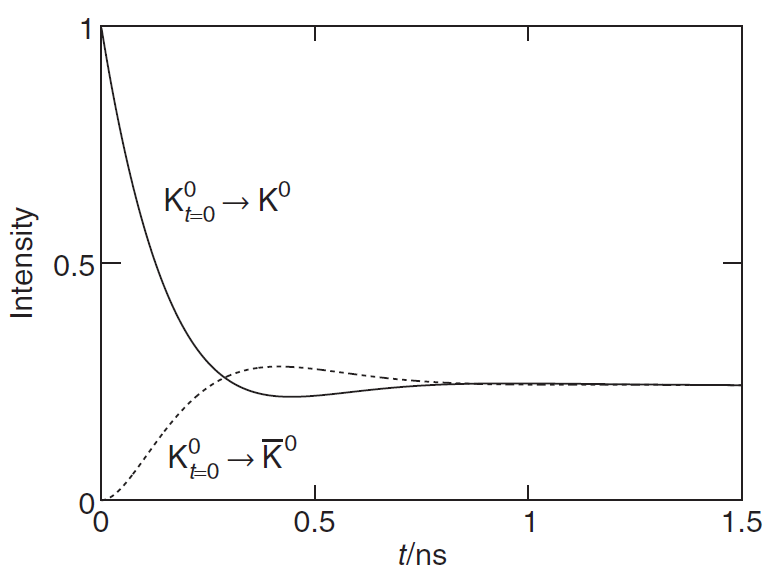
\includegraphics[width=0.65\textwidth]{C:/Users/Carmen/Desktop/Universidad/TFG/Borradores/img/osci2.PNG}
	\caption[Efecto de las oscilaciones de sabor en mesones $\PK$ neutros.]
	{Oscilaciones kaones neutros para un haz inicial puro de $\PKz$ \cite{Thomson}.}
	\label{fig:oscillation2}
\end{figure}